% ##################################################################################################################
\chapter{Samara}
\label{ch:samara}
\hfill \textbf{Authors:} Oleg Saprykin, Olga Saprykina, Tatyana Mikheeva

% ##################################################################################################################
\section{Study Area}
Samara is a major Russian city and the regional capital of the Samara region. The city is situated on the left bank of the Volga River, between the mouths of the rivers Samara and Sok. The area is 466\, square kilometers, nine administrative districts. Population of the city is 1\,172\,348 people (year~2014). There are more than 2.7\,million people live in a limit of the city agglomeration (GKS, 2010) \citep[][]{}.

Personal and public transports are developed within the city of Samara. Auto-mobilization of the population is 286\,vehicles per 1\,000\,people (year~2014) (Gradoteka, 2015) \citep[][]{}. Public transport is represented by trams, buses, trolleybuses and subway. Transit of freight transport through the city is prohibited.

Samara is a major economic, transport, scientific, educational and cultural center. However, despite this, street and road network of the city is not developed well enough. In general, following problems can be denoted.

\begin{itemize}
\item Street and road network has only two highways, which are connected by narrow streets, transverse highways are absent. It leads to the traffic congestion formation in the city. According to researches of Yandex company, Samara city was identified to fourth place by quantity of traffic jams among the Russian cities (Yandex Company, 2013) \citep[][]{}.
\item Lack of sufficient parking areas leads to a forced parking along the roads of the city, which creates additional traffic congestion.
\item Active development of the construction segment in~2000, which characterized by absence of city building general strategy, led to the obvious violations in transport planning, and significantly degrade the quality of transport infrastructure.
\item Samara is located opposite the Samarskay Luka National Park, surrounded by the unique beauty of natural places. This contributes to a huge number of recreational trips made during summer weekends. So this fact leads to uneven distribution of traffic flows in the region.
\end{itemize}

In addition to these problems, the Samara city is tending to sustainable development at the moment, which raises new challenges:
\begin{itemize}
\item rapid growth of residential development within the city boundaries requires modification of the transport infrastructure,
\item formation of new neighborhoods and new cottage villages within the urban agglomeration involves the construction of new roads, bridges and interchanges,
\item carrying out of the World Cup FIFA-2018 requires the organization of traffic management in the downtown area, the stadium area and the festival fans area.
\end{itemize}

Indicated issues and development trends require modernization of street and road network. It is impossible without supporting the projects by traffic flow simulation modeling.

% ##################################################################################################################
\section{Transport Demand}
Coordinates of the population residence places were taken from the anonymized information about the city population spatial distribution provided by the National Population Census~2010 (GKS, 2010) \citep[][]{}. Coordinates of employment places were taken as data about the organizations from the Samara region companies and organizations address directory.

Statistic package R was used for calculation of \gls{od} matrices. Collected information about population distribution and employment places were used as initial data. The estimation of \gls{od} matrices was performed by the entropy model that uses Shelehovsky-Shtskiy balance method (Nurminski et al., 2009; Autodor, 2013; Shvetsov, 2003) \citep[][]{}. This approach is applicable for estimation of the \gls{od} matrices values in case worker, business or recreation trips for private vehicles or freight transport. As a result the \gls{od} matrix was obtained, which showed quantity of the agents moving from one transport zone to another.

Activity chains were calculated for define path of each \gls{matsim} agent. Calculation of the activity chains was performed by especially developed method using the author's algorithm that described in (Saprykina, 2012) \citet[][]{}. The activity chains calculation uses \gls{od} matrices as source data. The resulted data was kept in the plans file and used in \gls{matsim}.

% ##################################################################################################################
\section{Transport Supply}
As shown in Figure~\ref{fig:samara_fig1}, the road network was extracted from \gls{osm} and saved to the \gls{matsim} network format using the \lstinline|NetworkEditor| module presented in Section~\ref{sec:contrib-networkEditor}. 
%\ah{Ref. which one?} \ah{according to Oleg's mail it was the ``old'' editor} 
Detailed verification of the obtained network mod-el showed up that some roads have incorrect number of lanes. This required writing a utility that semi-automatically allowed adjusting the street and road network model according to the actual transportation planning scheme. Minor inaccuracies of the model were corrected manually in the \lstinline|NetworkEditor|. The final network model consists of 4\,365\,nodes and 11\,178\,links.
%
 %------------
\createfigure%
{The transport network extraction process}%
{The transport network extraction process}%
{\label{fig:samara_fig1}}%
{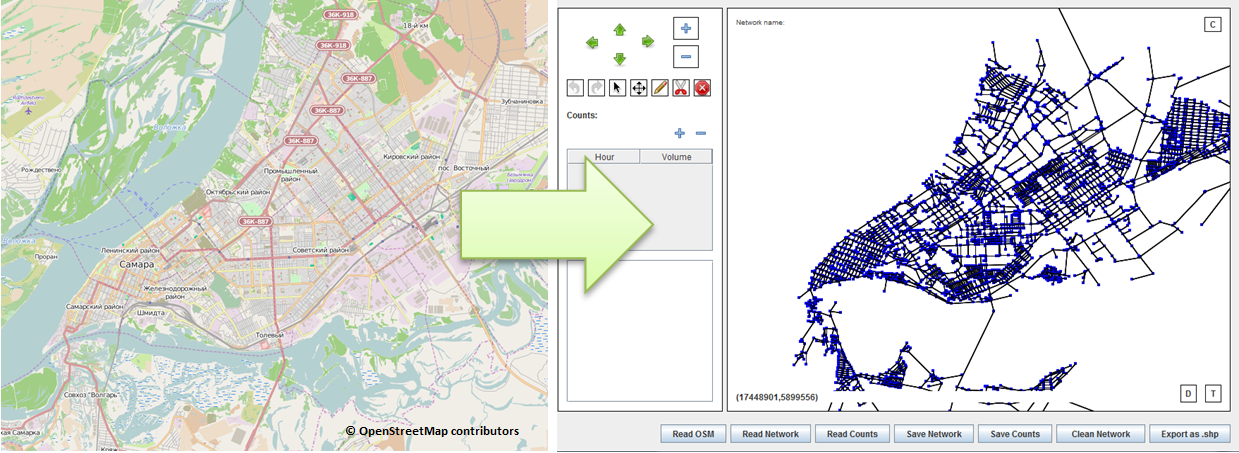
\includegraphics[width=0.99\textwidth, angle=0]{./scenarios/figures/samara_fig1.png}}%
{}
 %------------

The network model should contain elements of the transport infrastructure for adequate reflection of transportation planning. The model takes into account some traffic signs: speed limit, traffic lanes, movement on the interceptions, ``no entry''. Addition of traffic lights to the model is under development now. At this point schemes of traffic light regulation at certain intersections are developed and work on their integration into the general city model is underway.

Transport simulation was performed only for private vehicles. Inclusion of public transport to the model is under development at present. Bicycle paths are still poorly developed in the city there-fore their simulation is the low-priority task. 

% ##################################################################################################################
\section{Calibration and Validation}
For calibration purposes information about traffic flows at all intersections of Krasnoglinskoye highway and Voljskoe highway, as well as at the intersections of central (historical) part of the city, was used. Traffic flow intensity data was received for the period from 19th to 24th of May~2009. Source data required preprocessing, which consist in alignment of vehicles number according to their type and calculation of the total intensity in the target area. The requirement for the maxi-mum intensity was complied due to the fact that the intensity measurements were performed in the ``rush hours'' from 8\,am to 11\,am and from 4\,pm to 7\,pm (Mikheeva, 2008) \citep[][]{}. 

For validation of the transport infrastructure model and verification of its adequacy to the real traffic conditions in the city, following steps were completed: 
\begin{itemize}
\item field measurements of traffic flow parameters,
\item gathering data from different traffic Web-services (Yandex Maps, Google Maps, etc.),
\item comparative analysis of results obtained from the simulation, field explorations and Web-services (Saprykina, 2014) \citep[][]{}.
\end{itemize}

% ##################################################################################################################
\section{Intelligent Traffic Analysis}
During solving the applied problems the simulation results analysis is especially valuable. 
With \gls{matsim}'s tools Senozon \gls{via} (Chapter~\ref{ch:via}) and \gls{otfvis} (Chapter~\ref{ch:otfvis}) visual analysis of the model can be done. 
However, a deeper understanding of the model can be achieved by applying data mining tools to the simulation results. 
This will identify hidden patterns and correlations that will give more information for addressing applied problems. 

After the simulation output folder contains files with events and actual plans, containing all actions performed by agents. For loading the data to the mathematical package R performed converting them to \lstinline|.csv| format by specially designed utility and MS Excel application. Transport infrastructure information from external sources was also imported to R as a table containing the coordinates and types of the object. This made it possible to process the MATSim output using all power of the programming language R.

Searching for hidden patterns was performed using the \lstinline|NeuralNet| package installed in R. One of the goals was finding dependencies of tension at the gravity points of transport flows from the spatio-temporal parameters of transport infrastructure. For solving this problem was used feed-forward neural network, trained by resilient back-propagation with weight backtracking algorithm. Source data were split into training and test sets in a ratio 70/30. Verification was carried out by the regularity criterion (Mikheeva, 2012) \citep[][]{}.

The result of the study is the trained neural network, which able to predict the tension of the gravity points during the transport infrastructure parameters changing. This eliminates the need restarting the simulation to test the hypotheses for city transport infrastructure changes, allowing seeing the result of changes on the fly. Figure~\ref{fig:samara_fig2} shows the tension calculation process at the intersection by the trained neural network.

 %------------
\createfigure%
{The tension calculation process by the trained neural network}%
{The tension calculation process by the trained neural network}%
{\label{fig:samara_fig2}}%
{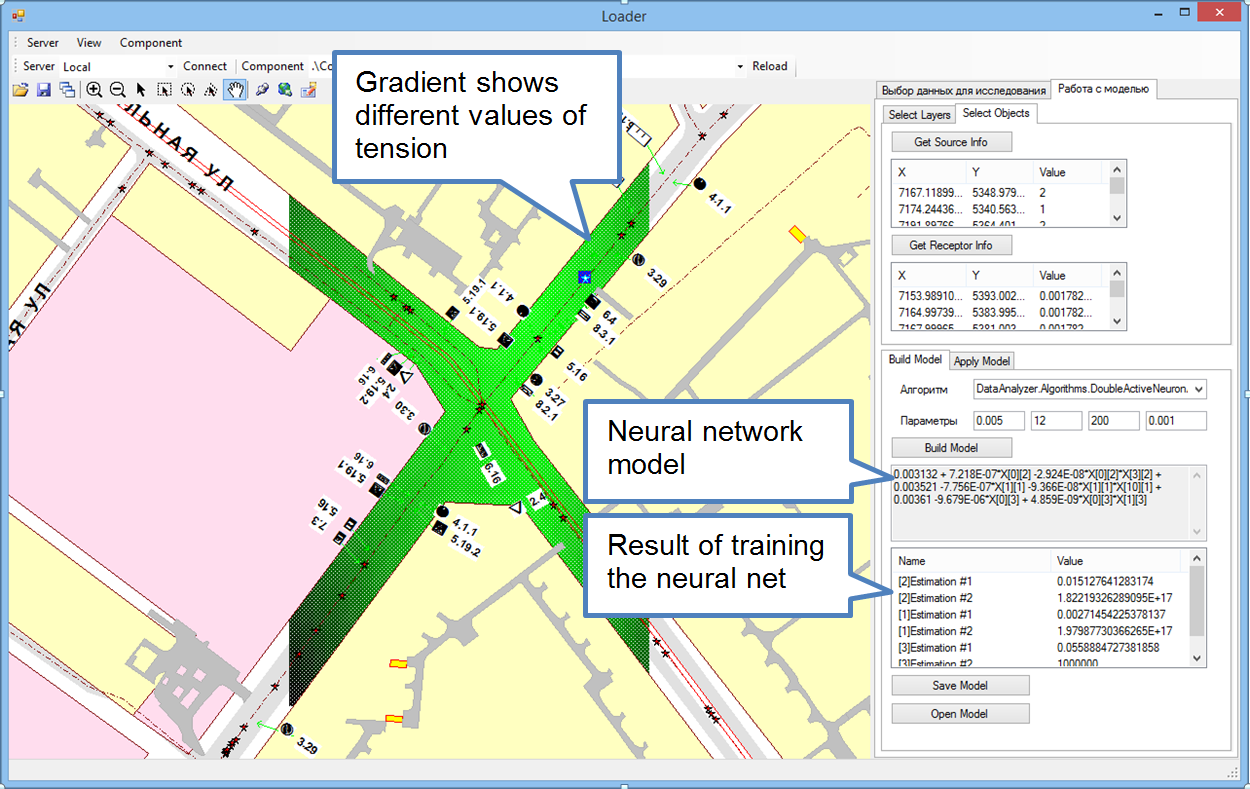
\includegraphics[width=0.99\textwidth, angle=0]{./scenarios/figures/samara_fig2.png}}%
{}
 %------------

% ##################################################################################################################